\documentclass[a4paper]{report}
 
\usepackage{graphicx}
\usepackage{url}
\usepackage{subcaption}
\usepackage[section]{placeins} % Ensure floats do not go into the next section
\usepackage{rotating} % For rotating figures, tables, etc. Including their captions

\begin{document}
	\title{Overview of anime voice actor's social network and popularity.}
	\author{Florencia Zanollo. Hideaki Takeda.}
	\maketitle
	\tableofcontents

\begin{abstract}
	Although Social Network of actors is a relatively common object of investigation that has been addressed many times, we can say that seiyuu (anime voice actors) come from a very different industry with a distinct way to relate to each other. \\
	In this research we use Wikidata and MyAnimeList to collect seiyuu information and build a Social Network. Topics explored:
	\begin{itemize}
	\item Structure and characteristics of seiyuu Social Network.
	\item Understanding what properties have a main role describing and predicting popularity of seiyuu.
	\item Compare prediction performances between different machine learning algorithms (and different models).
	\end{itemize}
\end{abstract}

\chapter{Introduction}
	TODO

% Main Part
\chapter{Anime/Seiyuu Dataset}

TODO DIVIDIR UN POCO MAS ESTA PARTE EN SUBSECTIONS Y AGREGAR MAS INFO O MUESTRAS DE DATOS

Wikidata\footnote{http://wikidata.org/} is a collaboratively edited knowledge base intended to provide a common source of data which can be used by Wikimedia projects such as Wikipedia. The information is stored in RDF format, and can be retrieved in multiple ways, one of them being through a SPARQL endpoint.

Using Wikidata's SPARQL endpoint we retrieved a list of seiyuu. This list contains all persons that have seiyuu as occupation, a total of 6472 entities were obtained\footnote{There's actually 7030 seiyuu in Wikidata but only 6472 of them have an English label (name)}. Gender, birthday and birthplace information was also fetched (last two were not used in the end because it was lacking in the majority of entities).

Since Wikidata information about seiyuu's works is really incomplete, MyAnimeList (MAL)\footnote{https://myanimelist.net/} was used to retrieve voice acting roles and anime information. MAL is a social networking and social cataloging application website with a large database on anime and manga that started in April 6, 2006. Users can make a list of currently watching, watched and/or favorite anime; score, review, comment and recommend similar ones. They can also comment about and favorite people working on the industry (voice actors, directors, editors, etc).\\


Since only 59 of Wikidata's seiyuu entities had MyAnimeList ID (MALID) property, a matching between Wikidata and MyAnimeList was done using seiyuu's complete name to retrieve the ID for those who was missing. Successfully restoring 3033 MALIDs, giving a total of 3092 seiyuus with that property; 2956 of them having at least one work according to MAL so we are using this subset for our experiments.

Using Jikan API\footnote{https://jikan.docs.apiary.io/\#} and MALID, seiyuu data, voice acting roles and more information about each anime was retrieved. 

An issue to take into account is whether we unify all anime adaptations of the same intellectual property as one or take a single adaptation as a independent work. We chose the later because each adaptation has its own producer, score, popularity, among other information; it would be incorrect to say a seiyuu worked in a popular work when that adaptation didn't have enough fame.\\

Information used:
\begin{itemize}
	\item For Seiyuu:
	\begin{itemize}
		\item Name
		\item Debut (this was obtained from oldest work aired date)
		\item Gender
		\item Popularity (member\_favorites information of MAL)
		\item Work (anime roles)
	\end{itemize}
	\item For Works (Anime):
	\begin{itemize}
		\item Year that began airing
		\item Favorites
		\item Score (from 0 to 10, MAL user based)
		\item Popularity (ranking over all MAL animes)
		\item Members (how many MAL users have it on their list)
		\item Genres
	\end{itemize}
\end{itemize}

It's important to notice that data such as popularity and scores are retrieved from MAL, which is user review based only; it may differ with actual awards winning or professional reviewing of works.

Further, this dataset is biased in favor of more recent anime and seiyuu, since it accounts for more complete data and with better quality. Oldest anime in this dataset is from 1960 having no record about previous ones. Majority of seiyuu's debut are from 1988 which leads us to think information from thereon is more complete. 

The data was stored using Virtuoso server to create a local SPARQL endpoint, mongodb was also used as an intermediate storage (before formatting data as RDF).












\chapter{Seiyuu Social Network}
Social networks consist of a finite set of actors and the relations between them. Usually represented as a graph; with actors or organizations as set of nodes and a defined relation between them as set of edges. This structures are useful to analyze complex social interactions and communities.

\section{Node and edge definitions}
This social network is of a particular kind called \textit{two-mode networks} which consists of a set of actors (seiyuu) and events (anime). So there exists two ways of viewing it, one will be from seiyuu perspective, using anime in common for edges; the other being from anime perspective, using seiyuu in common for edges. We chose the former since we found more interesting they being actual people and using other information about them such as debut and gender.

So our social network consists of voice actors as nodes and co-workership between them as edges. It's important to notice that this social network is time dependant since each seiyuu has a debut year and each anime has an aired time; giving us freedom to choose different time frames to observe.

Aside from being time dependant there exists different possible definitions of relationship or co-workership between seiyuu. One could say two actors know each other if they have worked in at least one job together, or maybe it requires more than one. There's also a time frame to define, relationship could take into account all works of both of them or only from certain years.\\

\section{Construction}
As a first approach Gephi was used to build the network. Since the graph was big enough to bring performance problems and we needed to build the edges dynamically (which couldn't be done in Gephi) NetworkX was used instead.

NetworkX was chosen because it's an easy yet powerful Python library, it doesn't get along with massive graphs but ours was not big enough to present a problem. 

One can export the graph and open it on Gephi, for a more visual analysis.

And also we needed to build the edges dynamically because according to our definition they depend on the time frame we are looking at. For example, for at least 10 works in common, if two actors worked together in 9 jobs between 1960 and 1970 we shouldn't see an edge between them; but if they worked together again in 1971 then looking at 1960-1971 they should be connected.

\section{Analysis}
In this section we are going to compare and analyze two definitions of relationship for our social network in order to understand more about it structure and decide on a definition:
\begin{itemize}
\item at least 1 work in common
\item at least 10 works in common
\end{itemize}
Both of them during the time frame between the first debut registered (1960) and the year of observation.

Is easy to tell at first glance that this social network is really interconnected. With merely 2956 nodes it has 395887 edges when only one work in common is required and 13629 edges when asking for 10 or more. It shows a thightly interconnected cluster surrounded by poorly or not connected nodes. This cluster represents 99\% of the nodes of one work in common graph and 23\% of 10 works in common. In terms of modularity we can see at least four clear communities in each graph, Fig~\ref{fig:graph1CommunityColoured} and Fig~\ref{fig:graph10CommunityColoured}.

\begin{figure}[!hbt]
	\begin{center}
	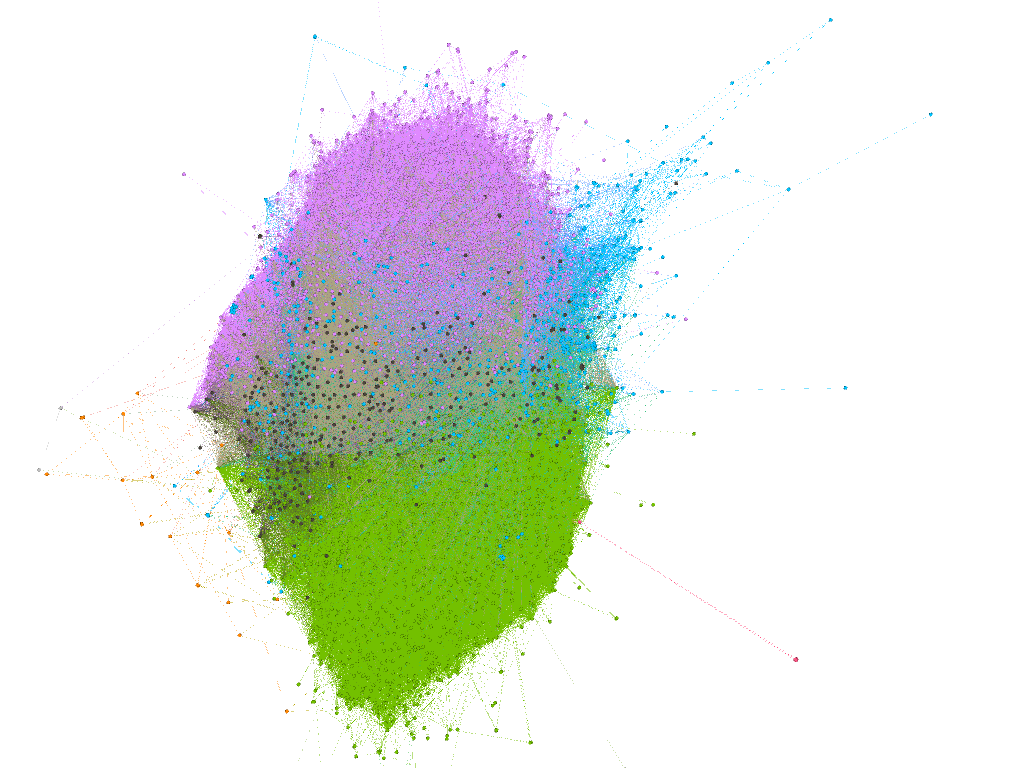
\includegraphics[width=\columnwidth]{graphics/atLeast1WorkCommunity.png}
	\caption{At least one work in common graph coloured by community.}
	\label{fig:graph1CommunityColoured}
	\end{center}
\end{figure}

\begin{figure}[!hbt]
	\begin{center}
	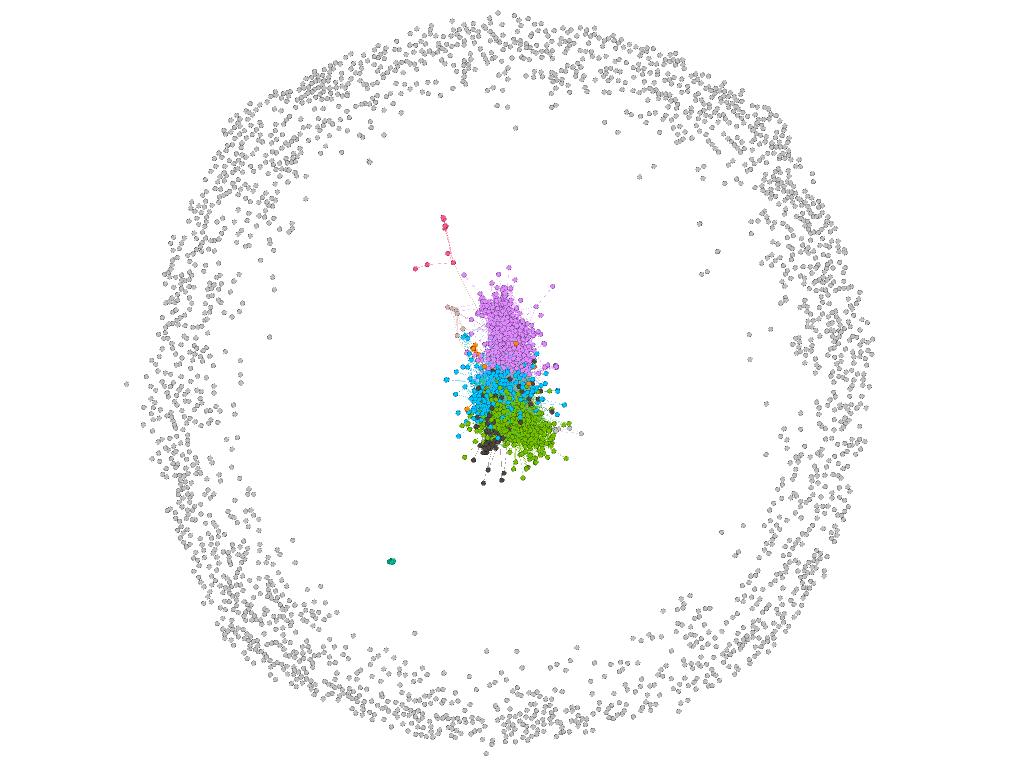
\includegraphics[width=\columnwidth]{graphics/atLeast10WorksCommunity.png}
	\caption{At least ten works in common graph coloured by community. Big cluster at the center, surrounded by loosely connected nodes.}
	\label{fig:graph10CommunityColoured}
	\end{center}
\end{figure}

Table~\ref{tab:graphComparision} shows metrics about each graph. Requiring more works in common decreases average degree circumstantially but doesn't change much modularity or network diameter.

\begin{table}[!hbt]
	\begin{center}
	\caption{Graph analysis}
	\label{tab:graphComparision}
	\begin{tabular}{|l|c|c|c|}
		\hline
		Graph & Avg Degree & Graph Density & Modularity \\
		\hline
		One work in common & 267 & 0.09 & 0.2 \\
		\hline
		Ten works in common & 9 & 0.003 & 0.29 \\
		\hline
	\end{tabular}\\
	\smallskip
	\begin{tabular}{|l|c|c|}
		\hline
		Graph & Network Diameter & Connected Components \\
		\hline
		One work in common & 6 & 18 \\
		\hline
		Ten works in common & 7 & 2261 \\
		\hline
	\end{tabular}
	\end{center}
\end{table}

\begin{figure}
	\centering
	\begin{subfigure}{.5\columnwidth}
		\centering
		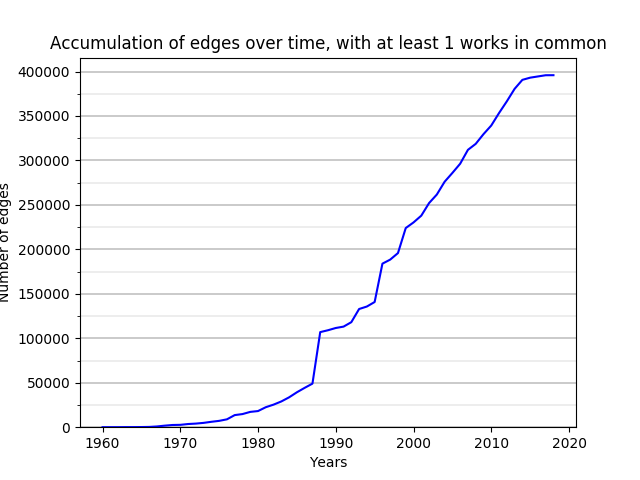
\includegraphics[scale=0.39]{graphics/accumulationEdges_1_1960-2018.png}
		\caption{At least one work in common}
		\label{fig:edgesOneWorkInCommon}
	\end{subfigure}%
	\begin{subfigure}{.5\columnwidth}
		\centering
		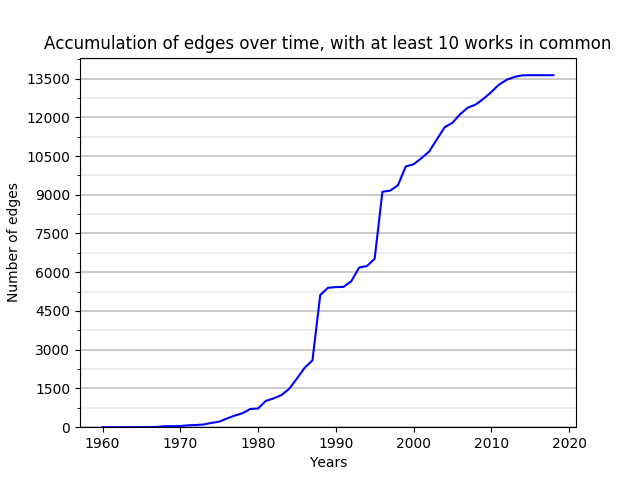
\includegraphics[scale=0.39]{graphics/accumulationEdges_10_1960-2018.png}
		\caption{At least ten works in common}
		\label{fig:edgesTenWorskInCommon}
	\end{subfigure}
	\caption{Grouwth of edges over time. For 1 and 10 works in common graphs}
	\label{fig:grouwthOfEdges}
\end{figure}

As proven by Fig.~\ref{fig:grouwthOfEdges} grouwth of edges by year follows a similar distribution regardless of how many works in common are used to build the social network.

\begin{figure}[!hbt]
	\begin{center}
	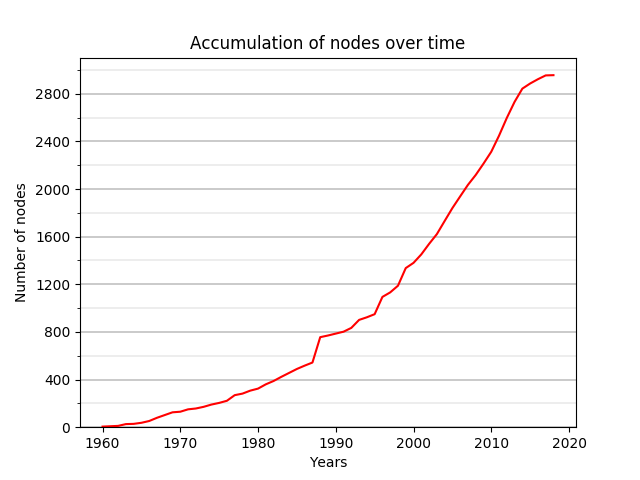
\includegraphics[width=\columnwidth]{graphics/nodesAccumulation.png}
	\caption{Grouwth of nodes over time.}
	\label{fig:grouwthOfNodes}
	\end{center}
\end{figure}
 
Fig.~\ref{fig:grouwthOfNodes} shows that more than half of the nodes are from last 18 years (2000 to 2018), giving us an idea of how much seiyuu industry is growing.

\FloatBarrier
Table~\ref{tab:top10atLeast1Work} shows top 10 nodes, for degree and betweenness centrality for "at least 1 work in common" definition. And Table~\ref{tab:top10atLeast10Works} does the same for "at least 10 works in common".

\begin{table}[!htb]
    \begin{minipage}{.5\textwidth}
        \centering
            \begin{tabular}{|l|c|}
				\hline
				Name & Degree \\ 
				\hline
				Takehito Koyasu & 1545 \\ 
				\hline
				Akira Ishida & 1488 \\ 
				\hline
				Mamiko Noto & 1422 \\ 
				\hline
				Nobuo Tobita & 1417 \\ 
				\hline
				Daisuke Namikawa & 1390 \\ 
				\hline
				Nobuyuki Hiyama & 1358 \\ 
				\hline
				Rikiya Koyama & 1331 \\ 
				\hline
				Jūrōta Kosugi & 1322 \\ 
				\hline
				Keiji Fujiwara & 1312 \\ 
				\hline
				Kazuhiko Inoue & 1309 \\ 
				\hline
			\end{tabular}
            \caption{Top 10 degree}
    \end{minipage}%
    \begin{minipage}{.6\textwidth}
        \centering
        \begin{tabular}{|l|c|}
				\hline
				Name & Betweenness Centrality \\
				\hline
				Takehito Koyasu & 49982.52 \\
				\hline
				Akira Ishida & 40221.50 \\
				\hline
				Daisuke Namikawa & 30448.43 \\
				\hline
				Nobuo Tobita & 29363.25 \\
				\hline
				Mamiko Noto & 29168.18 \\
				\hline
				Rie Kugimiya & 29122.31 \\
				\hline
				Miyuki Sawashiro & 28997.40 \\
				\hline
				Kazuhiko Inoue & 27693.88 \\
				\hline
				Daisuke Ono & 27034.592 \\
				\hline
				Keiji Fujiwara & 26802.69 \\
				\hline
		\end{tabular}
        \caption{Top 10 Betweenness centrality }
    \end{minipage}
    \caption{At least one work in common}
    \label{tab:top10atLeast1Work}
\end{table}

\begin{table}[!htb]
    \begin{minipage}{.5\textwidth}
        \centering
            \begin{tabular}{|l|c|}
				\hline
				Name & Degree \\
				\hline
				Takehito Koyasu & 311 \\
				\hline
				Akira Ishida & 273 \\
				\hline
				Mamiko Noto & 258 \\
				\hline
				Daisuke Namikawa & 232 \\
				\hline
				Katsuyuki Konishi & 229 \\
				\hline
				Keiji Fujiwara & 220 \\
				\hline
				Junichi Suwabe & 216 \\
				\hline
				Toshiyuki Morikawa & 215 \\
				\hline
				Rie Kugimiya & 213 \\
				\hline
				Nobuyuki Hiyama & 201 \\
				\hline
			\end{tabular}
            \caption{Top 10 degree}
    \end{minipage}%
    \begin{minipage}{.6\textwidth}
        \centering
        \begin{tabular}{|l|c|}
				\hline
				Name & Betweenness Centrality \\
				\hline
				Takehito Koyasu & 18489.44 \\
				\hline
				Mamiko Noto & 10988.96 \\
				\hline
				Daisuke Namikawa & 9570.48 \\
				\hline
				Akira Ishida & 8299.19 \\
				\hline
				Rie Kugimiya & 7560.16 \\
				\hline
				Katsuyuki Konishi & 7413.72 \\
				\hline
				Kenichi Ogata & 7160.54 \\
				\hline
				Harumi Sakurai & 6775.76 \\
				\hline
				Keiji Fujiwara & 5980.58 \\
				\hline
				Yoshimasa Hosoya & 5607.95 \\
				\hline
		\end{tabular}
        \caption{Top 10 Betweenness centrality }
    \end{minipage}
    \caption{At least ten works in common}
    \label{tab:top10atLeast10Works}
\end{table}

\section{Summarization}
Both networks have fairly similar top 10s so it points to them having similar structure and connections amoung their nodes, aside from actual values.\\

From now on our definition for edges will be: \textit{at least 10 works in common, during the time frame between the first debut registered (1960) and the year of observation}. Because requiring more jobs in common means less amount of edges, this leaves a more understandable graph and we verified it does without changing its structure so much.\\

There's also other interesting definitions of relationship, for example we can use only common works from the last x years or from all time. This options weren't explored; having into account our limited time.\\

Table~\ref{tab:moreInfoSeiyuu} shows a little more information about seiyuu that appear on top 10s.
\begin{table}[!hbt]
	\begin{center}
	\caption{More information about seiyuu appearing in top 10 lists}
	\label{tab:moreInfoSeiyuu}
	\begin{tabular}{|l|c|c|c|c|}
		\hline
		Name & Popularity & Debut & Gender & Birthyear \\
		\hline
		Takehito Koyasu & 7235 & 1988 & Male & 1967 \\
		\hline
		Akira Ishida & 7612 & 1989 & Male & 1967 \\
		\hline
		Mamiko Noto & 7544 & 1988 & Female & 1980 \\
		\hline
		Daisuke Namikawa & 8304 & 1988 & Male & 1976 \\
		\hline
		Katsuyuki Konishi & 3702 & 1996 & Male & 1973 \\
		\hline
		Keiji Fujiwara & 2778 & 1986 & Male & 1964 \\
		\hline
		Junichi Suwabe & 10838 & 1996 & Male & 1972 \\
		\hline
		Toshiyuki Morikawa & 2455 & 1981 & Male & 1967 \\
		\hline
		Rie Kugimiya & 31668 & 1996 & Female & 1979 \\
		\hline
		Jun Fukuyama & 26811 & 1981 & Male & 1978 \\
		\hline
		Kenichi Ogata & 52 & 1974 & Male & 1942 \\
		\hline
		Harumi Sakurai & 341 & 2005 & Female & 1982 \\
		\hline
		Yoshimasa Hosoya & 4852 & 2006 & Male & 1982 \\
		\hline
		Nobuo Tobita & 139 & 1981 & Male & 1959 \\
		\hline
		Nobuyuki Hiyama & 1723 & 1988 & Male & 1967 \\
		\hline
		Rikiya Koyama & 2919 & 1996 & Male & 1963 \\
		\hline
		Jūrōta Kosugi & 114 & 1985 & Male & 1957 \\
		\hline
		Miyuki Sawashiro & 26501 & 1988 & Female & 1985 \\
		\hline
		Kazuhiko Inoue & 2445 & 1974 & Male & 1954 \\
		\hline
		Daisuke Ono & 24080 & 1996 & Male & 1978 \\
		\hline
	\end{tabular}
	\end{center}
\end{table}

\section{Afterwork}
By the end of the research we were able to grab new information about seiyuu roles; we now know if it was a main role (mostly main character or villian) or not.

Giving this new information we built another social network using the following definition of relationship:\\

\textit{At least one work in common, during the time frame between the first debut registered (1960) and the year of observation, \textbf{using information from  main roles only}.}\\

We'll now present some characteristics of this network.

\begin{figure}[!hbt]
	\begin{center}
	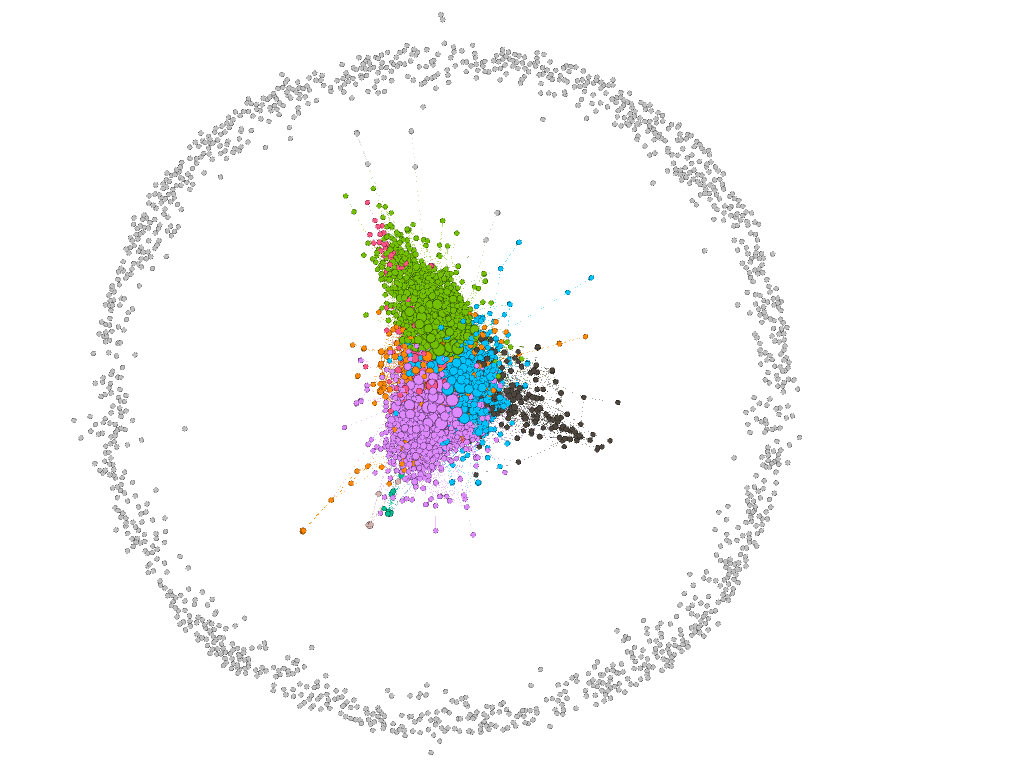
\includegraphics[width=\columnwidth]{graphics/atLeast1WorksOnlyMainRoleCommunity.png}
	\caption{At least one "main role" work in common graph coloured by community. It also has a big cluster at the center.}
	\label{fig:graph1MWCommunityColoured}
	\end{center}
\end{figure}

As Fig.~\ref{fig:graph1MWCommunityColoured} shows this graph's structure is also a strongly connected cluster surrounded by loosely or not connected nodes. Then Table~\ref{tab:newGraphAnalysis} has some features of this network.

\begin{table}[!hbt]
	\begin{center}
	\caption{Graph analysis}
	\label{tab:newGraphAnalysis}
	\begin{tabular}{|l|c|c|c|}
		\hline
		Graph & Avg Degree & Graph Density & Modularity \\
		\hline
		Only main works & 14 & 0.005 & 0.355 \\
		\hline
	\end{tabular}\\
	\smallskip
	\begin{tabular}{|l|c|c|}
		\hline
		Graph & Network Diameter & Connected Components \\
		\hline
		Only main works & 8 & 1349 \\
		\hline
	\end{tabular}
	\end{center}
\end{table}


\section{Analysis and prediction of seiyuu popularity}

\PARstart{P}{opularity} is an abstract criterion that must be defined as a numerical metric in order to be used for analysis and prediction. Since we are using MAL database for seiyuu and anime information and it has a social component; seems logic to use member\_favorites as a representation of popularity. We can also get popularity and score for works from opinions of the same set of users.

In terms of distribution \textit{popularity} is highly unequal \---as we can observe in Fig.~\ref{fig:popularityDistribution}\--- having a lot of seiyuu which are no member favourites and only a few who are favorite of more than 10000 members. It's good to keep in mind that users can favorite multiple seiyuu.

\begin{figure}[!hbt]
	\begin{center}
	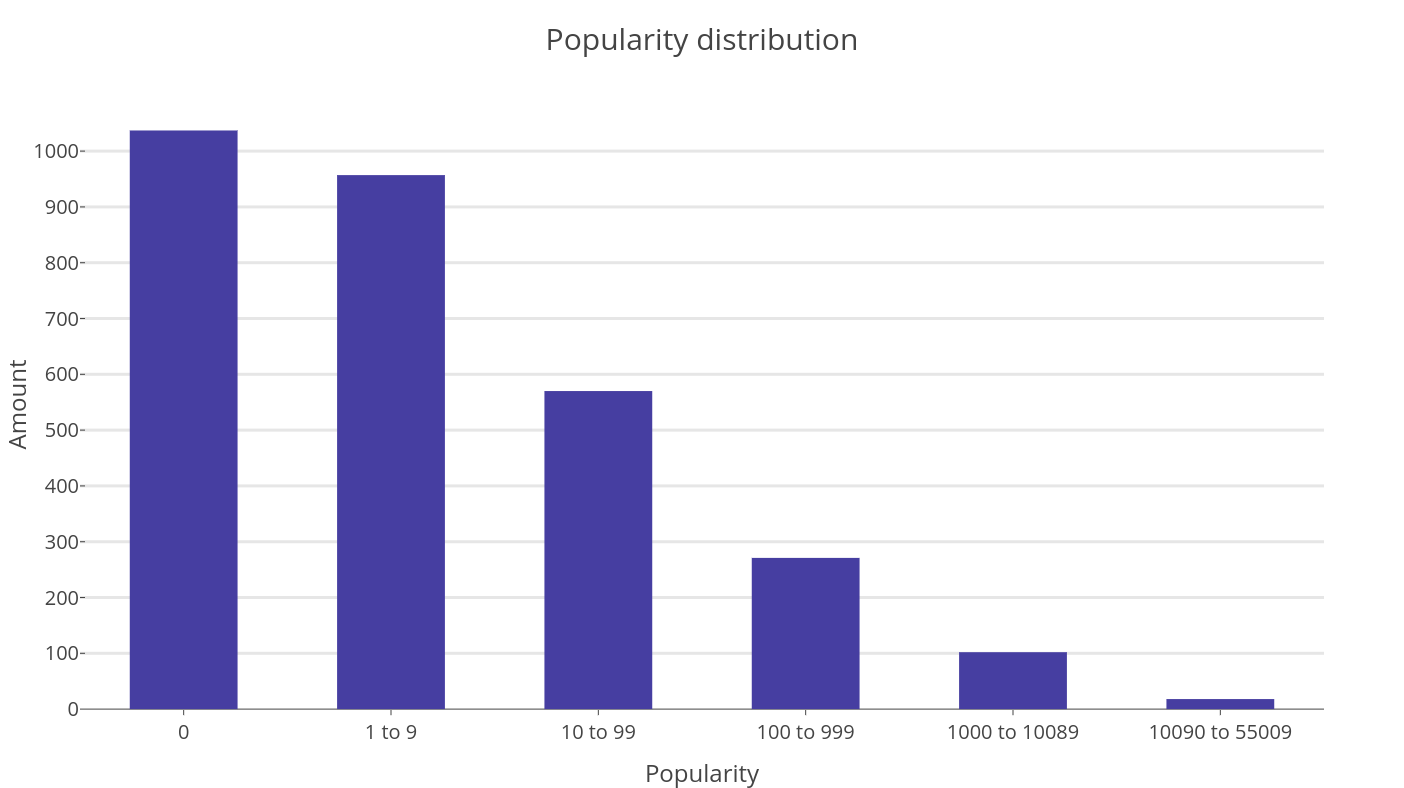
\includegraphics[width=\columnwidth]{graphics/popularityDistribution.png}
	\caption{Amount of seiyuu with that popularity, divided into groups for better visualization.}
	\label{fig:popularityDistribution}
	\end{center}
\end{figure}

This is something to take into account when trying to predict popularity of actors or explain it using other features. TODO ADD WHY

\begin{itemize}
	\item Mean:    289.55
	\item Median:    2.0
	\item Max:    55018
	\item Min:    0 (1037 values equal to zero)
	\item Only 120 values bigger than 1000
\end{itemize}

\subsection{Correlation with only one feature}
First approach to explaining popularity was using Pearson’s correlation. 

TODO PEARSON'S GRAPHIC

A fairly big correlation can be seen between popularity and amount of works. Since this data is biased to more modern anime we thought of trying to correlate with more recent works only. But, how recent? Last 5, 10 or 20 years? Thus correlation between popularity and works from different data frames was analyzed, Fig.~\ref{fig:correlationPopRecentWorks}.

\begin{figure}[!hbt]
	\begin{center}
	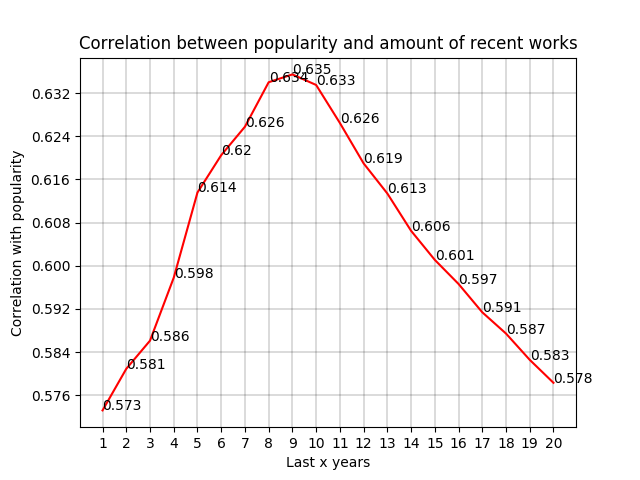
\includegraphics[width=\columnwidth]{graphics/correlationPopRecentWorks.png}
	\caption{Last \textit{X} years means works from 2018-\textit{X} to present.}
	\label{fig:correlationPopRecentWorks}
	\end{center}
\end{figure}

The best result was given by recent works from last 9 years. Therefore this definition of recent works was used from there on.

Graphics of some characteristics of works divided by years were made, trying to shed some light over why works from last 9 years were more "important". TODO EXPLANATION OF EACH FIGURE AND RE-WRITE THIS PART: 
- looking at graphs Fig.~\ref{fig:avgCaracteristicsOfWorks} it seems avg popularity, favorites and score of anime from last 9 years is not better that previous, actually is worst. but as we can see on Fig.~\ref{fig:amountOfWorksPerYear} they are more, anime industry is growing bigger each year, in a exponential way, not only that but MAL should have info of every adaptation of last year but maybe not for anime from 1980.

The majority of works are from 1990 to 2018 and half of them are distributed over the last 14 years (2014 to 2018) but as far as we can tell there isn’t anything particular over the last 9 years nor on year 2009.

\begin{figure}[!hbt]
	\begin{center}
	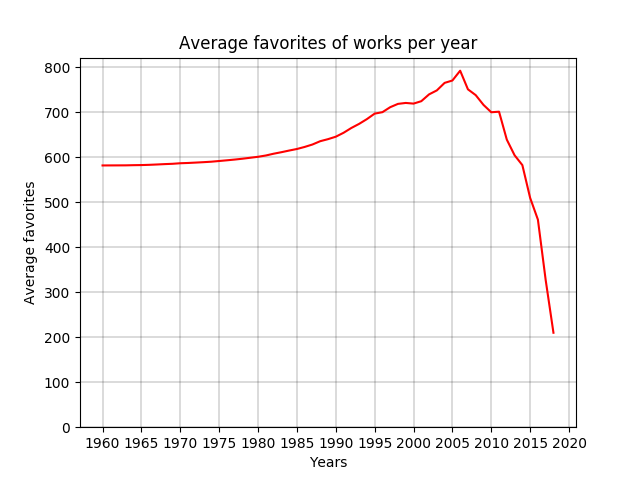
\includegraphics[width=\columnwidth]{graphics/avgFavoritesPerYear_1960-2018.png}
	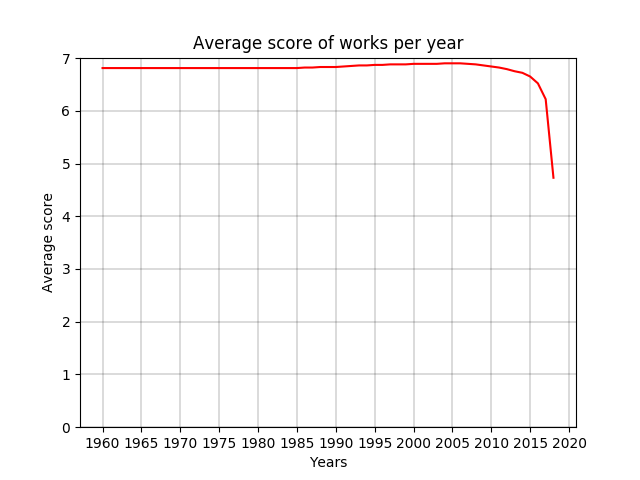
\includegraphics[width=\columnwidth]{graphics/avgScorePerYear_1960-2018.png}
	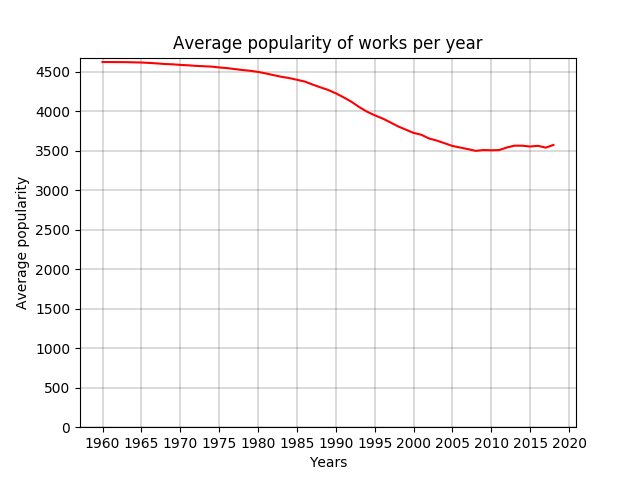
\includegraphics[width=\columnwidth]{graphics/avgWorksPopularityPerYear_1960-2018.png}
	\caption{TODO ADD DESCRIPTION.}
	\label{fig:avgCaracteristicsOfWorks}
	\end{center}
\end{figure}

\begin{figure}[!hbt]
	\begin{center}
	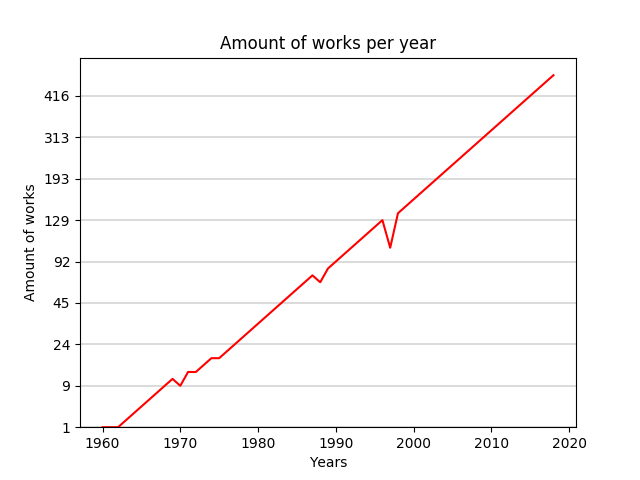
\includegraphics[width=\columnwidth]{graphics/worksPerYear_1960-2018.png}
	\caption{Amount of works divided by years which were aired for the first time.}
	\label{fig:amountOfWorksPerYear}
	\end{center}
\end{figure}

Some interesting enough correlations are shown next
TODO ADD SCATTER PLOTS AND EXPLAIN A LITTLE MORE

\subsection{Correlation with multiple features}
For this section Scikit-learn, a free software machine learning Python library, was used. The node attributes were divided into categories, leaving four distinct types:

\begin{itemize}
	\item Personal data:
	\begin{itemize}
		\item Debut
		\item Gender
		\item Activity years (2018-debut)
	\end{itemize}
	\item Works data:
	\begin{itemize}
		\item Amount
		\item Top 5 genre
		\item Favorites
		\item Score
		\item Popularity
	\end{itemize}
	\item Recent works data:
	\begin{itemize}
		\item Same as works but for only last 9 years
	\end{itemize}	
	\item Graph data:
	\begin{itemize}
		\item Degree
		\item Betweenness centrality
		\item Closeness
	\end{itemize}
\end{itemize}

Fitting and prediction experiments were run for each category, each combination of 2, 3 and all of them together; using 80\% as train data and the rest as test. This was done for all following models:
\begin{itemize}
	\item DecisionTreeRegressor
	\item DecisionTreeClassifier
	\item LinearRegression
	\item KNeighborsClassifier
	\item LinearDiscriminantAnalysis
	\item GaussianNB
	\item SVM
\end{itemize}

TODO, WRITE THIS AGAIN:
To compare prediction performance mean and median absolute error were used. Unfortunately since popularity variance is really high we observed good results in terms of absolute error but particular predictions were aloof. That's why we ended up using r2\_score for accuracy comparation. 

TODO SHOW TABLE WITH R2 SCORE RESULTS FOR EACH CATEGORY / MODEL AND GROUP OF CATEGORIES






\chapter{Conclusion}
	

\begin{thebibliography}{5}
	%Each item starts with a \bibitem{reference} command and the details thereafter.

\end{thebibliography}

\end{document}